\documentclass[conference]{IEEEtran}

% --- Paquetes esenciales ---
\usepackage[utf8]{inputenc}
\usepackage[english]{babel}
\usepackage{graphicx}
\usepackage{amsmath}
\usepackage{booktabs}
\usepackage{array}
\usepackage{geometry}
\usepackage{hyperref}
\usepackage[numbers]{natbib}  % Usa [numbers] si prefieres citas numeradas
\geometry{margin=1in}

% --- Título y autores ---
\title{Deterministic Random Bit Generators: A Comparison of NIST-Approved Techniques}

\author{
    Tomas Bedoya \\
    Daniel Andres Jaimes Cárdenas \\
    Eder Leandro Carbonero Baquero \\
    \textit{Universidad de los Andes, Colombia}
}

\date{\today}
\pagestyle{plain} 
% --- Documento principal ---
\begin{document}

\maketitle

\begin{abstract}
The following paper centers around several methods of random number generation. It aims to comprehend the essential concepts behind RNG, including pseudo and true random generation. Additionally, it explores different approaches to randomness that are used today following the NIST SP 800-90 standards, both reliant on entropy sources as well as algorithmic techniques, and compares their randomness with a series of statistical tests to determine which operate better and suggest appropriate uses for the different methods.
\end{abstract}

\begin{IEEEkeywords}
CTR DRBG, Counter mode Deterministic Random Bit Generator, NIST, National Institute of Standards and Technology, AES, Advanced Encryption Standard, RBG, Random Bit Generator, DRBG, Deterministic Random Bit Generator, RNG, Random Number Generator, PRNG, Pseudorandom Number Generator, TRNG, True Random Number Generator, DRNG, Digital Random Number Generator, ENRNG, Enhanced Random Number Generator, HSM, Hardware Security Module
\end{IEEEkeywords}

\section{General Definitions}
\noindent
With the aim of providing a broader understanding of the various concepts addressed in this document, the following are definitions of some of the acronyms that will be mentioned throughout the text.
% genericos.tex

\begin{table}[h!]
\centering
\begin{tabular}{@{}ll@{}}
\toprule
\textbf{Acronym} & \textbf{Meaning} \\ \midrule
CTR\_DRBG & Counter mode Deterministic Random Bit Generator \\
NIST & National Institute of Standards and Technology \\
AES & Advanced Encryption Standard \\
RBG & Random Bit Generator \\
DRBG & Deterministic Random Bit Generator \\
PRNG & Pseudorandom Number Generator \\ \bottomrule
\end{tabular}
\caption{Acronyms definitions.}
\label{tab:acronyms}
\end{table}

\section{Introduction}
Due to the deterministic nature of traditional computers, which is what most people and appliances use to this day and will continue being so for the foreseeable future, Random Number Generation (RNG) has proven to be a challenge. Due to the reliance of cryptographic algorithms, communication protocols and other security systems in random values, there’s a constant race to find ever-better sources of randomness that follow the international standards of quality; the higher the randomness of a source, the greater the security it provides. This proves to be a challenge, however, for true randomness is difficult to find. Computers themselves cannot produce it and rely on Pseudo Random Number Generation (PRNG) to simulate random values. Other techniques, such as finding random measurements on certain like the time between user key strokes or mouse movements have proven to be unsatisfactory when put under statistical scrutiny (Mechalas, 2018). 
To guarantee that sensible processes utilize proper random sources, the NIST structured the SP 800-90 Standards for Random Number Generation (RNG) for safe RNG in cryptographic contexts. The following sections delve deep into several RNG methods, both of pseudo and true randomness, that follow these standards. They explore the different entropy sources they use (or don’t), analyses how they extract random number chains from them, and evaluate the quality of their randomness through a series of statistical evaluations. Our aim is to understand better where RNG stands today, to evaluate how they fare against each other, and determine which of these methods work better for which applications.


As discussed in \cite{nist800-90a}, the NIST standards provide a comprehensive framework for deterministic random bit generators.

\section{Key Concepts}
Most RNG methods can be classified into one of two categories. The first of these is Pseudo Random Number Generation, sometimes called Deterministic Random Bit Generation (DRBG) (Cao et al., 2022). A PRNG is a deterministic algorithm that produces numbers that appear to be random. It requires a seed value to generate a seemingly random number, and due to its deterministic nature, the same seed will produce the same value every time. PRNGs experience periodicity, for after exhausting all possible internal variations, it will repeat cycles that will reiterate on the sequences of produced numbers. Good PRNG algorithms, however, manage to display good statistical behaviors, with some having periods in order of magnitudes so large they become negligible. Due to their algorithmic nature, PRNGs are quick and scalable; their deterministic nature is also desirable in experiments where replicability is key. However, they are extremely unsafe key producers for cryptographic measures, for a backtrack of the algorithm or the knowledge of the seed reveal the output in its entirety  (Mechalas, 2018). 
True Random Number Generators (TRNG), on the other hand, aim to produce true random values. To achieve this, TRNG relies on entropy sources, which extract true randomness by extracting information from physical phenomena. The two main types of entropy sources are dynamic entropy sources, which extract true random values from indeterminate physical processes like thermal noise or atmospheric noise, and static entropic sources, which extract randomness from randomly occurring properties in the hardware components of the computer as a result of the semiconductor manufacturing process, which become stable once the device is finished. These properties can be found in chip and are used for things like authentications (Cao et al., 2022). What is essential is that an entropy source extracts its randomness from the physical world, which means that no “randomness” generated by a procedural method can be considered an entropy source. TRNGs are desirable where safety is essential, and show constant distributions that guarantee unpredictability, but are usually slow to output a number due to their need to measure physical phenomena; this takes time and is computationally costly, which makes them not very scalable.
Some methods can be classified into particular categories of RNG.  Cascade Construction Random Number Generator (CCRNG), for example, relies on an entropy source to supply an “entropy buffer”, which is then used to provide cryptographically secure PRNG. Digital Random Number Generators (DRNGs) is an approach that builds the RNG on the processor’s hardware directly, and uses a combination of CCRNG and dynamic entropy sources to create random streams. Even so, this categories are usually some sort of combination of PRNG and TRNG to different degrees, and combining both methods is becoming more common in the industry to tackle the strengths and weaknesses of both methods.


\section{Studied Methods}
The following RNG methods are the ones that will be seen in detail for the rest of this report.
\section{Methology}
\subsection{Random Number Generation}
\label{sec:random_generation}

For this exercise, three different forms of random number generation were performed. The first was through the \textit{CTR\_DRBG} algorithm, which used random keys generated by the \texttt{random} function of the Python programming language version 3.9 as seeds and was executed on a MacBook Pro M3 Pro computer. This detail may lead to different results if the experiment is replicated. However, we assume that Python's \texttt{random} function generates a uniform randomness distribution, simulating an entropic system for generating random bits.

For the second option, a sequential range of seeds was chosen, which were formatted in 32 bits to ensure compatibility with AES encryption. The sequence started at 1 and increased by one until reaching 50 million seeds. These seeds were then used to execute the \textit{CTR\_DRBG} algorithm, which generates the pseudo-random bit values.

The third approach made use of the Beacon system. In this case, the official NIST API was consumed to retrieve the last 15,600 random bits, generated from 512-bit values, obtained from the historical records maintained by the system.


\section{Statistical Testing}
Due to their protagonic relevance in cryptography and security, as mentioned before, the evaluation of random and pseudorandom number generators (RNGs/PRNGs) is a critical aspect of their deployment. The statistical properties of the generated sequences must approximate those of true random sequences to ensure unpredictability and reliability. The National Institute of Standards and Technology (NIST) Special Publication 800-22 Rev 1a provides a widely recognized suite of statistical tests for this purpose, offering tools to detect deviations from randomness in binary sequences. While no finite set of tests can provide absolute certification of randomness, these tests serve as an essential initial step in assessing a generator's suitability.

The five tests selected from the NIST suite for this analysis---Frequency (Monobit) Test, Frequency Test within a Block, Runs Test, Maurer's "Universal Statistical" Test, and the Cumulative Sums (Cusum) Test---were chosen to provide a balanced and comprehensive assessment. This selection emphasizes tests that are both fundamental in their approach and offer insights into different potential weaknesses of an RNG, ranging from basic distributional properties and sequential dependencies to more complex characteristics like data compressibility, which relates to the sequence's entropy. The aim is to cover a diverse range of statistical attributes with tests that are also relatively accessible in their conceptual underpinnings, facilitating a clear interpretation of a generator's performance.

\smallskip

\textbf{Selected Statistical Tests: Description and Interpretation}

\smallskip

\subsection{\textbf{Frequency (Monobit) Test}}

The \textbf{Frequency (Monobit) Test} is the most fundamental test, examining the overall proportion of zeros and ones in the entire binary sequence. Its purpose is to determine if the number of ones and zeros in a sequence are approximately equal, as would be expected for a truly random sequence. The test assesses the closeness of the fraction of ones to $1/2$ by converting the bits into a sequence of $+1$ and $-1$ values, summing these values to obtain $S_n$, and then computing a test statistic $s_{\text{obs}} = |S_n| / \sqrt{n}$. A P-value is subsequently calculated using the complementary error function, $P\text{-value} = \text{erfc}(s_{\text{obs}} / \sqrt{2})$. If the computed P-value is less than the chosen significance level $\alpha$ (typically $0.01$), the sequence is considered non-random; otherwise, it is considered random with respect to this test. A small P-value suggests that the sum $S_n$ is too large, indicating an excess of ones or zeros in the sequence. NIST recommends a minimum sequence length of 100 bits for this test.

\subsection{\textbf{Frequency Test within a Block}}

The \textbf{Frequency Test within a Block} focuses on the proportion of ones within M-bit blocks of the sequence. Its objective is to determine whether the frequency of ones in an M-bit block is approximately $M/2$, as would be expected under an assumption of randomness. The input sequence is partitioned into $N = \lfloor n/M \rfloor$ non-overlapping blocks. For each block, the proportion of ones ($\pi_i$) is calculated, and a $\chi^2$ statistic is computed as $\chi^2(\text{obs}) = 4M \sum_{i=1}^{N}(\pi_i - 1/2)^2$. The P-value is then determined using the incomplete gamma function ($\text{igamc}(N/2, \chi^2(\text{obs})/2)$). If the P-value is less than $\alpha$ (e.g., $0.01$), it suggests non-randomness, indicating that at least one block deviates significantly from the expected equal proportion of ones and zeros. Recommended input parameters include $n \ge 100$, $M \ge 20$, $M > 0.01n$, and $N < 100$.



\subsection{\textbf{Runs Test}}

The \textbf{Runs Test} examines the total number of runs in the sequence, where a run is defined as an uninterrupted sequence of identical bits. The purpose is to determine if the oscillation between zeros and ones is too fast or too slow, which would indicate a deviation from randomness. A prerequisite is that the sequence passes a basic frequency check: if the proportion of ones, $\pi$, satisfies $|\pi - 1/2| \ge \tau$, where $\tau = 2/\sqrt{n}$, the Runs Test is not performed. If applicable, the test statistic $V_n(\text{obs})$, the total observed number of runs, is calculated. The P-value is then $P\text{-value} = \text{erfc}(|V_n(\text{obs}) - 2n\pi(1-\pi)| / (2\sqrt{2n}\pi(1-\pi)))$. A P-value less than $\alpha$ (e.g., $0.01$) leads to the conclusion that the sequence is non-random. A large value of $V_n(\text{obs})$ suggests the oscillation is too fast, while a small value indicates it is too slow. A minimum sequence length of 100 bits is recommended.



\subsection{\textbf{Maurer's "Universal Statistical" Test}}

\textbf{Maurer's "Universal Statistical" Test} evaluates the compressibility of the sequence, focusing on the number of bits between matching L-bit patterns. The test aims to detect whether a sequence can be significantly compressed without loss of information; a significantly compressible sequence is considered non-random. The $n$-bit sequence is divided into an initialization segment of Q L-bit blocks and a test segment of K L-bit blocks. For each L-bit block in the test segment, the algorithm identifies the distance (in blocks) to its most recent previous occurrence found in the sequence processed so far. The test statistic, $f_n$, is the average of the base-2 logarithm of these distances over all K test blocks. This observed $f_n$ is compared to a theoretical expected value for the given L, $\text{expectedValue}(L)$, and a P-value is computed as $P\text{-value} = \text{erfc}(|f_n - \text{E}(L)| / (\sqrt{2}\sigma))$, where $\sigma$ is a pre-calculated standard deviation. If the P-value is less than $\alpha$ (e.g., $0.01$), the sequence is deemed non-random, suggesting it is compressible. This test requires long sequences, with L typically between 6 and 16, and $n$ chosen such that $K \approx 1000 \cdot 2^L$ and $Q = 10 \cdot 2^L$.

\subsection{\textbf{Cumulative Sums (Cusum) Test}}

The \textbf{Cumulative Sums (Cusum) Test} focuses on the maximal excursion (from zero) of a random walk defined by the cumulative sum of adjusted (-1, +1) digits in the sequence. The purpose is to determine if this cumulative sum is too large or too small relative to the expected behavior for random sequences. The (0,1) sequence is converted to a sequence of $X_i$ values of -1 and +1. Partial sums $S_k$ are computed. The test statistic $z$ is the maximum absolute value among these partial sums ($z = \max_{1 \le k \le n} |S_k|$). The test can be applied in a forward direction (mode=0) or a backward direction (mode=1). The P-value is calculated based on $z$ and $n$, involving sums of normal cumulative distribution function evaluations. If the P-value is less than $\alpha$ (e.g., $0.01$), the sequence is considered non-random. Large excursions suggest an excess of ones or zeros at the beginning (forward mode) or end (backward mode) of the sequence, while very small excursions might indicate that ones and zeros are intermixed too evenly. A minimum sequence length of 100 bits is recommended.

Additionally, we presented a visual test assesses byte sequence randomness by plotting a histogram of byte value frequencies (0-255). Ideally random data yields a flat, uniform histogram, as each byte value should occur with similar probability. Overlays like a normal distribution (using sample $\mu$ and $\sigma$) and highlighting extreme frequencies help visualize this. Significant deviations from uniformity, such as pronounced peaks or valleys, suggest potential non-randomness in the sequence.

\section{Results}
\subsection{Histogram analysis}
\label{sec:histogram_analysis}

\subsection{Distribution of Random Bits Generated with Python Random Seeds}
\label{sec:distribution_python_seed}

The distribution results of each technique are separated by the method used to obtain the seed versus the technique used to distill and obtain the random big number, so we can observe different results for each case.

To view the distribution of values, distribution graphs were used, either standard or uniform, depending on the input data. In our experiments, uniform distributions were shown. 8-bit segments were taken, dividing the entire input data set into byte blocks, obtaining bytes from 0 to 255. This range of possibilities gives us a visual of how the results are distributed.

We begin with the first technique, which was the generation of 6.25 million 32-byte seeds that were used to generate 6.25 million random bytes, or 50 million random bits, using the \textit{CTR\_DRBG} technique. The graph we see below leads us to the conclusion that there is a uniform distribution of the results without pronounced peaks, which are a symptom of an effective system in generating random bits.

\begin{figure}[htbp]
    \centering
    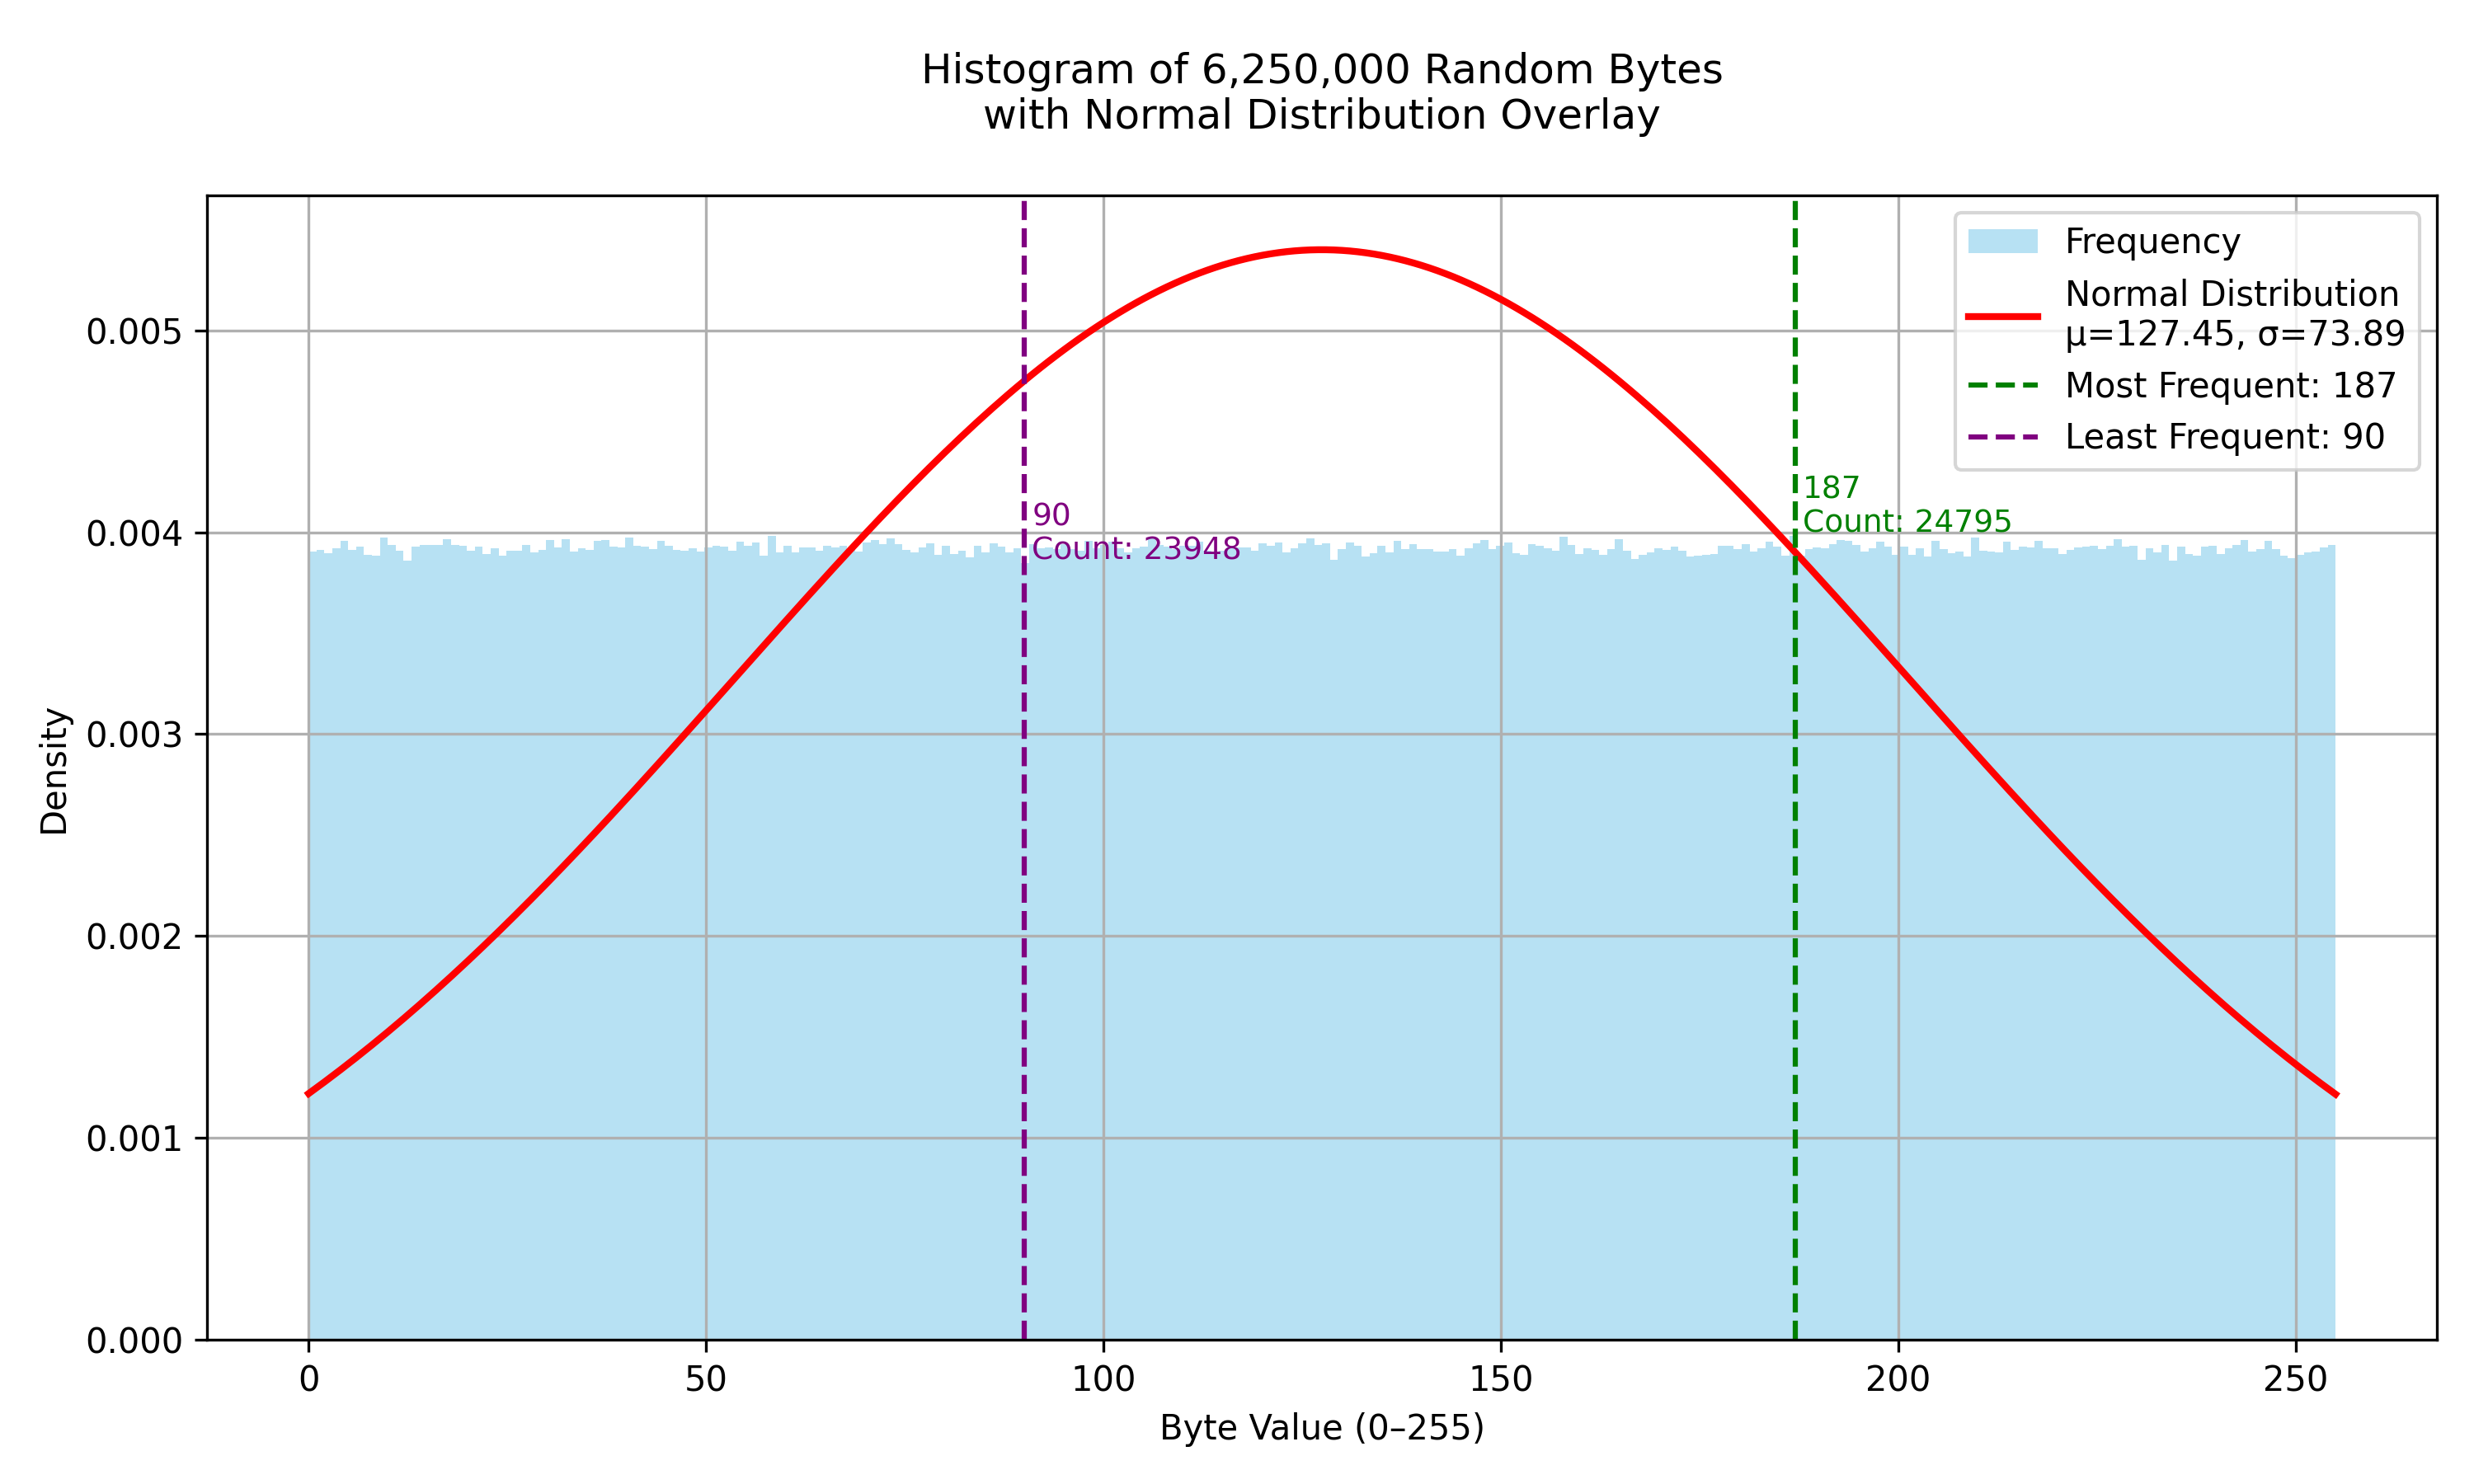
\includegraphics[width=0.9\linewidth]{images/random_bits_CTR_DRBG_seed_python_random.png}
    \caption{\raggedright Random bits \textit{CTR\_DRBG} seed generation with Python random function.}
    \label{fig:ctr_drbg_python_random}
\end{figure}


\subsection{Distribution of Random Bits Generated with Sequential Seeds}
\label{sec:distribution_sequential_seed}

For the following test, sequential seeds were used starting at 1 and reaching 6.5 million in the set of natural numbers. This number was converted to binary and turned into a 32-bit number, then it was used as a seed to generate the distribution with the \textit{CTR\_DRBG} method, showing a uniform distribution without much variation. Unexpectedly, it is seen that the distribution behaves very similar to obtaining reliable seeds with true entropy. Below is the graph.

\begin{figure}[htbp]
    \centering
    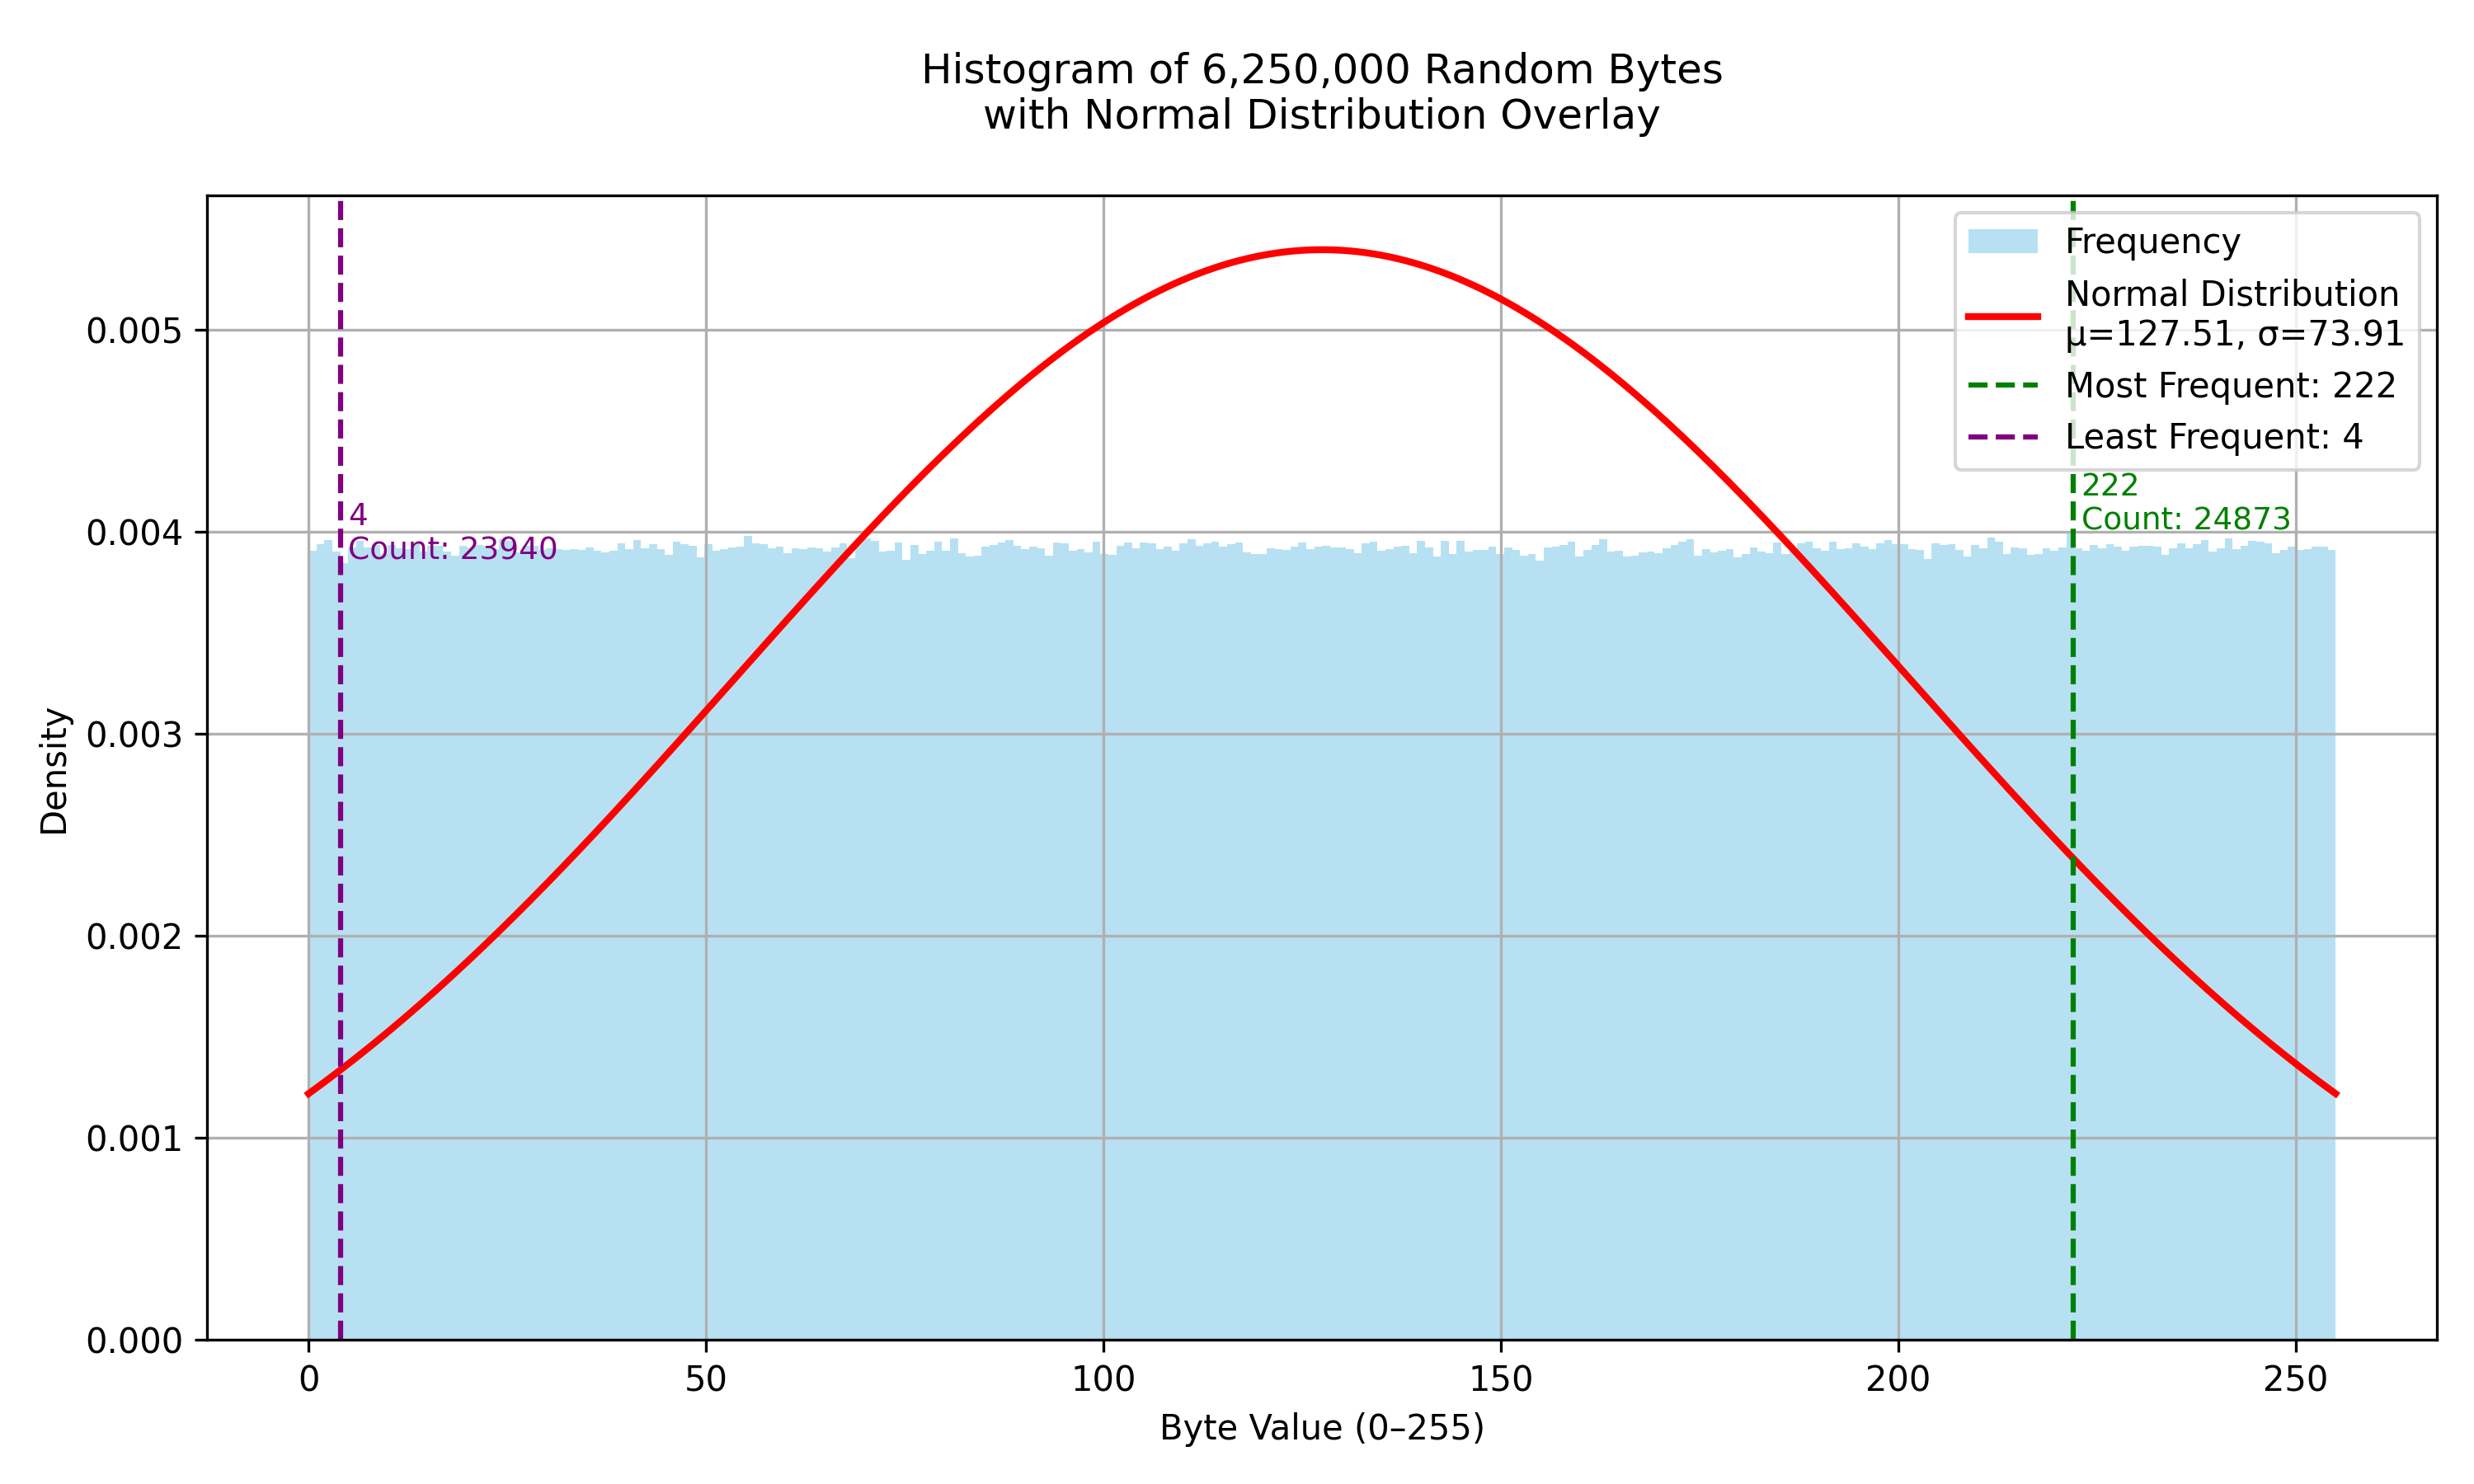
\includegraphics[width=0.9\linewidth]{images/secuentialSeedFrom0_To_100M_CTR_DRBG.png}
    \caption{\raggedright Sequential seed from 1 to 6.5M using \textit{CTR\_DRBG}.}
    \label{fig:ctr_drbg_sequential_seed}
\end{figure}


\section{Conclusions}
The comparative analysis of various random number generators, including classical pseudo-random (CRNG), Counter Mode Deterministic Random Bit Generators (CTR DRBG and CTR DRBG with sequential seeding), and a Quantum Random Number Generator (QRNG), was conducted using a selection of five statistical tests from the NIST SP 800-22 Rev 1a suite. These tests, namely the Frequency (Monobit) Test, Frequency Test within a Block, Runs Test, Maurer's "Universal Statistical" Test, and the Cumulative Sums (Cusum) Test, proved invaluable in assessing different aspects of randomness, from basic bit balance to compressibility and trend analysis . The results indicated that both CTR DRBG implementations exhibited excellent statistical properties, passing all applied tests and demonstrating characteristics consistent with high-quality random data suitable for cryptographic applications. In contrast, the evaluated QRNG, despite its theoretical underpinnings for true randomness, showed significant deviations, failing critical tests such as the Monobit, Runs, and Cusum tests, suggesting underlying biases or issues in the generation or collection process that compromise its statistical randomness for the tested 500,000-bit sequence. The classical RNG served as a baseline and generally performed well.


% OPCIÓN 1: Referencias con BibTeX
\bibliographystyle{plainnat}
\bibliography{references}  % Asegúrate de tener un archivo references.bib

\end{document}
